% !TEX root = ./beamer.tex
\documentclass[aspectratio=169]{beamer}
\usepackage[spanish]{babel}
\usepackage[utf8]{inputenc}
\usepackage{amsmath}
\usepackage{amssymb}
\usepackage{graphicx}
\usepackage{epstopdf}
\usepackage{rotating}
% \usepackage{cite}
\usepackage{color}
\usepackage{fancybox}
\usepackage{pstricks}
\usepackage{pst-plot}
\usepackage{pstricks-add}
\usepackage{epsf}

%\usepackage{apacite}
\usepackage[backend=biber,style=numeric, citestyle=ieee]{biblatex}
\addbibresource{references.bib} %Imports bibliography file

%Figuras
\usepackage{graphicx, subfigure}

%Matemática
\usepackage{amsmath}
\usepackage{amssymb}
\usefonttheme[onlymath]{serif}

%Algoritmos
\usepackage{float}
\usepackage{algorithm}
\usepackage{algorithmicx}
\usepackage{algpseudocode}

%Tema
\usetheme{Frankfurt}
\setbeamercolor{title}{fg=white, bg=black}
\usecolortheme{seagull}
\setbeamercolor{frametitle}{fg=white, bg=black}
\beamersetuncovermixins{\opaqueness<1>{10}}{\opaqueness<2->{15}}

%Opciones del tema
\setbeamertemplate{navigation symbols}{}
\setbeamertemplate{footline}[frame number]
\setbeamertemplate{caption}{\raggedright\insertcaption\par}

%citado de código
\usepackage{listingsutf8} % mejora compatibilidad con símbolos
\usepackage{inconsolata}
% Parámetros para las citas de código
\lstset{
    language=C++,
    basicstyle=\ttfamily\small,
    inputpath=scripts/,
    numberstyle=\footnotesize,
    numbers=left,
    backgroundcolor=\color{gray!20},
    frame=single,
    tabsize=2,
    rulecolor=\color{black!30},
    title=\lstname,
    commentstyle=\color{blue},
    keepspaces=true,
    %keywordstyle=\color{blue},
    stringstyle=\color{red},
    %escapeinside={\%*}{*)}
    breaklines=true,
    %breakatwhitespace=true, %Breaklines only in whitespaces. Comment for breaklines at any character.
    framextopmargin=2pt,
    framexbottommargin=2pt,
    inputencoding=utf8,
    extendedchars=true,
    literate={á}{{\'a}}1 {ü}{{\"u}}1 {é}{{\'e}}1 {í}{{\'i}}1 {ó}{{\'o}}1 {ú}{{\'u}}1 {ñ}{{\~n}}1
}

% Defines styling for C code listing
\definecolor{mGreen}{rgb}{0,0.6,0}
\definecolor{mGray}{rgb}{0.5,0.5,0.5}
\definecolor{mPurple}{rgb}{0.58,0,0.82}
\definecolor{backgroundColour}{rgb}{0.95,0.95,0.92}

\lstdefinestyle{CStyle}{
  backgroundcolor=\color{gray!20},
  commentstyle=\color{mGreen},
  keywordstyle=\color{magenta},
  numberstyle=\footnotesize,
  stringstyle=\color{mPurple},
  basicstyle=\ttfamily\small,
  breakatwhitespace=false,
  breaklines=true,
  keepspaces=true,
  numbers=left,
  frame=single,
  tabsize=2,
  rulecolor=\color{black!30},
  %escapeinside={\%*}{*)}
  framextopmargin=2pt,
  framexbottommargin=2pt,
  inputencoding=utf8,
  extendedchars=true,
  language=C
}

\usepackage{auto-pst-pdf}

\begin{document}
\title{Investigación bibliográfica: OpenACC}
\author{Willy Villalobos\\SP-2136 Programación Avanzada}


%Titulo
\begin{frame}
    \titlepage

    %\center{
\includegraphics[scale=0.05]{cnca.jpg}\\2015}\\
\end{frame}

%Tabla de contenidos
% \begin{frame}\frametitle{Contenidos}\tableofcontents
% \end{frame}

% \begin{frame}{Objetivo}
%     \begin{itemize}
%         \item Implementar el algoritmo de doble barrido para el etiquetado de imágenes en forma secuencial y en paralelo.
%         \item Realizar una comparativa del rendimiento de las implementaciones del algoritmo.
%     \end{itemize}
% \end{frame}

\begin{frame}{OpenACC}
    \begin{itemize}
        \item Modelo de programación basado en directivas, con una sintaxis similar a OpenMP.
        \item Inicialmente orientado al aprovechamiento de aceleradores. Podría considerarse un fork de OpenMP que poco a poco ha ido integrando las mismas características.
        \item Compatible con C, C++, Fortran.
    \end{itemize}
\end{frame}

\begin{frame}{OpenACC}
    \begin{itemize}
        \item Los pragmas tienen la siguiente sintaxis:
    \end{itemize}

    \begin{figure}
        \centering
        \subfigure[Sintaxis de pragmas]{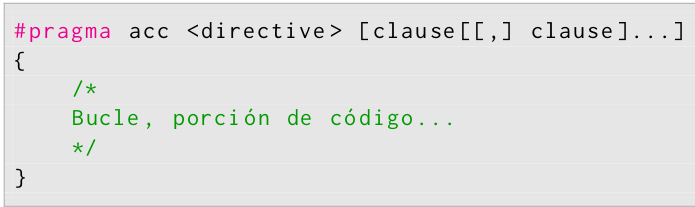
\includegraphics[scale=0.40]{01_pragma_syntax.png}}
    \end{figure}
\end{frame}

\begin{frame}{Tipos de directivas soportadas}
    \begin{itemize}
        \item Directivas de cómputo
        \item Directivas de manejo de datos.
        \item Directivas de sincronización.
    \end{itemize}
\end{frame}

\begin{frame}{OpenACC}
    \begin{itemize}
        \item Existe un API de OpenACC que extiende las capacidades de los pragmas:
    \end{itemize}

    \begin{figure}
        \centering
        \subfigure[Para importar el API y utilizar las características adicionales.]{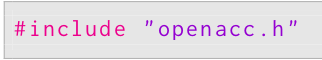
\includegraphics[scale=0.40]{02_import_api.png}}
    \end{figure}
\end{frame}

\begin{frame}{OpenACC}
    \begin{itemize}
        \item Los pragmas de kernels le indican al compilador cómo ejecutar el código según lo que indiquemos:
    \end{itemize}

    \begin{figure}
        \centering
        \subfigure[Directivas kernels, parallel/parallel loop]{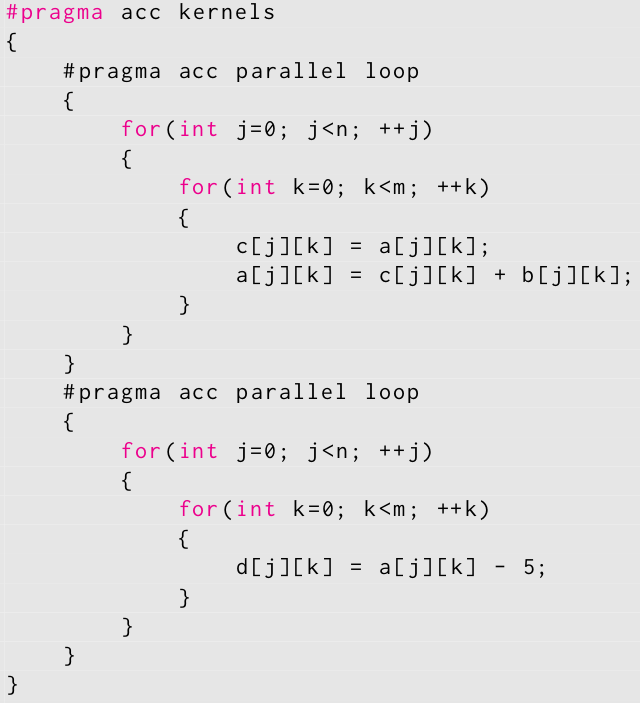
\includegraphics[scale=0.20]{03_kernels_parallel.png}}
    \end{figure}
\end{frame}

\begin{frame}{OpenACC}
    \begin{itemize}
        \item Las directivas de rutina se emplean para acelerar funciones específicas.
    \end{itemize}

    \begin{figure}
        \centering
        \subfigure[Directivas de rutina]{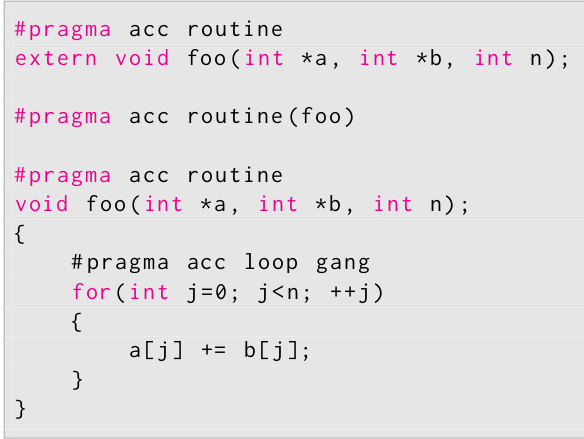
\includegraphics[scale=0.35]{04_routine_directives.png}}
    \end{figure}
\end{frame}

\begin{frame}{OpenACC}
    \begin{itemize}
        \item El compilador de PGI tiene un uso y sintaxis similares a GCC:
    \end{itemize}

    \begin{figure}
        \centering
        \subfigure[Compilación usando PGI.]{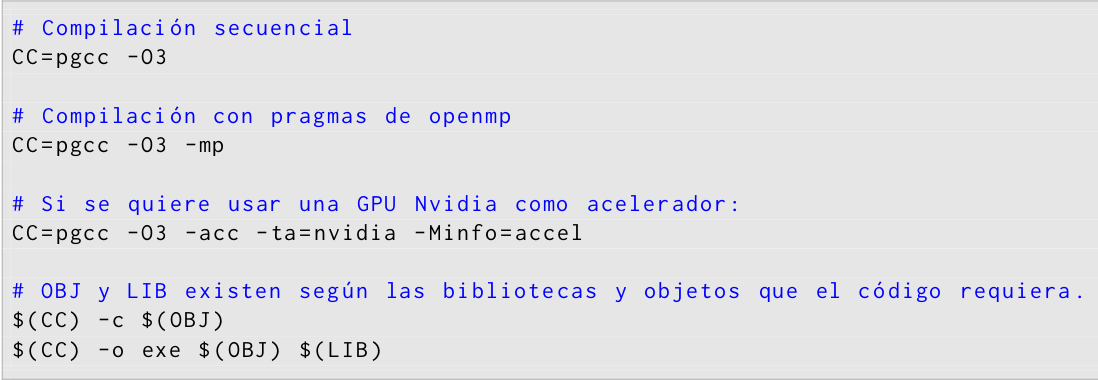
\includegraphics[scale=0.30]{05_compile.png}}
    \end{figure}
\end{frame}

\begin{frame}{OpenACC}
    \begin{itemize}
        \item El algoritmo para el área del conjunto de Mandelbrot emplea varios bucles for anidados.
    \end{itemize}

    \begin{figure}
        \centering
        \subfigure[Bucles de algoritmo de área de conjunto de Mandelbrot]{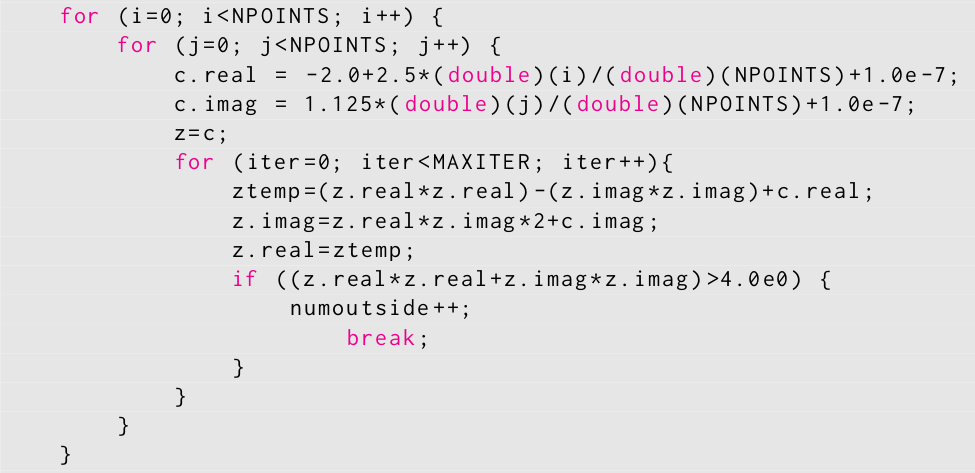
\includegraphics[scale=0.28]{06_original.png}}
    \end{figure}
\end{frame}

\begin{frame}{OpenACC}
    \begin{itemize}
        \item Para acelerar el código en este caso se emplearon los pragmas de parallel y loop.
    \end{itemize}

    \begin{figure}
        \centering
        \subfigure[Pragmas empleados para acelerar código.]{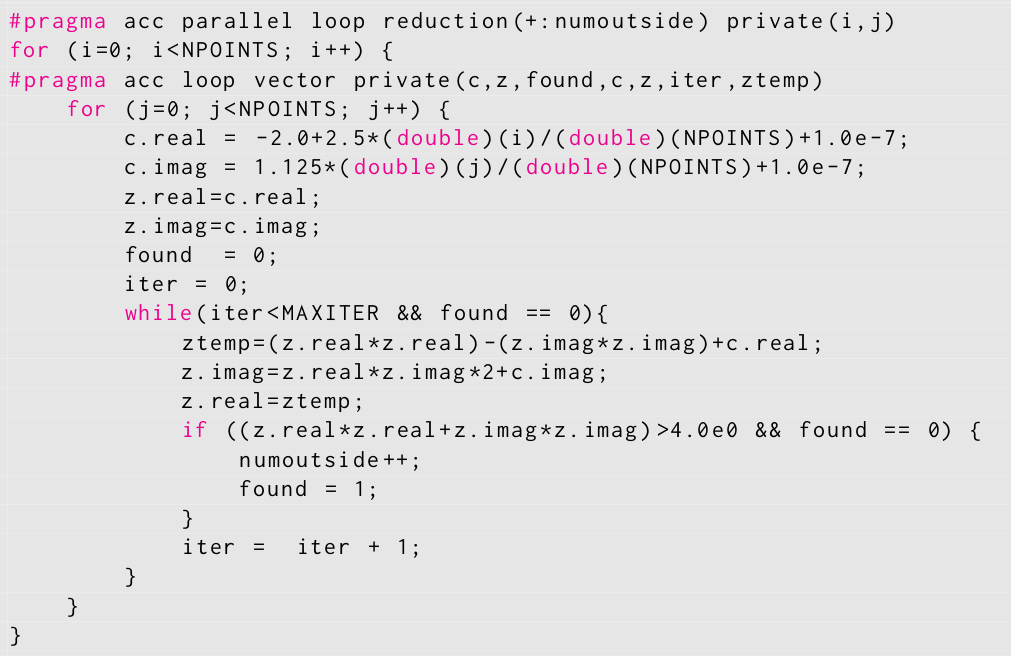
\includegraphics[scale=0.25]{07_used_pragmas.png}}
    \end{figure}
\end{frame}

\begin{frame}{OpenACC}
    \begin{itemize}
        \item Del código de prueba para el cálculo del área del conjunto de Mandelbrot, se obtuvieron estos resultados.
    \end{itemize}

    \begin{figure}
        \centering
        \subfigure[Resultados secuencial, OpenMP 4 threads, OpenACC GPU.]{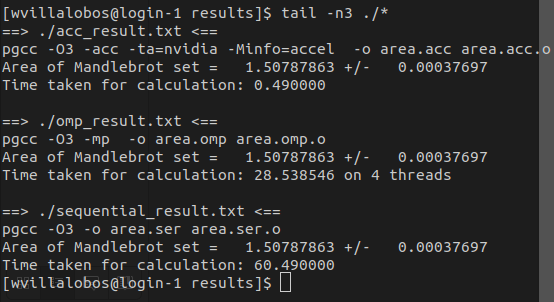
\includegraphics[scale=0.40]{08_results.png}}
    \end{figure}
\end{frame}

% \begin{frame}{Algoritmo Two-pass / Double-pass}
%     \begin{itemize}
%         \item Conocido también como algoritmo Hoshen-Kopelman.
%         \item Realiza un doble barrido sobre la imagen. La primera vez asigna etiquetas temporales y registra las equivalencias.
%         \item El segundo barrido reemplaza las etiquetas temporales por el valor más pequeño posible.
%         \item Se evalúan diferentes condiciones para actualizar o mantener la etiqueta de cada región en la imagen.
%     \end{itemize}
% \end{frame}

% \begin{frame}{Algoritmo Two-pass / Double-pass}
%     \begin{figure}
%         \centering
%         \subfigure[Etiquetado primer barrido]{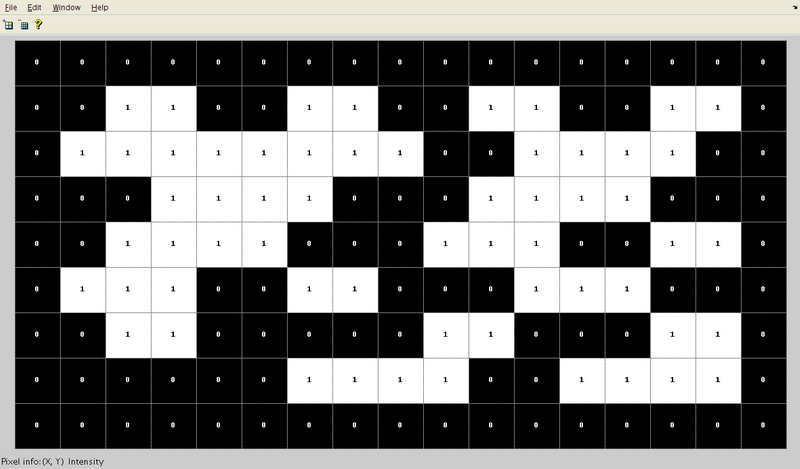
\includegraphics[scale=0.20]{Screenshot-Pixel_Region_(Figure_1).png}}
%         \subfigure[Etiquetado segundo barrido]{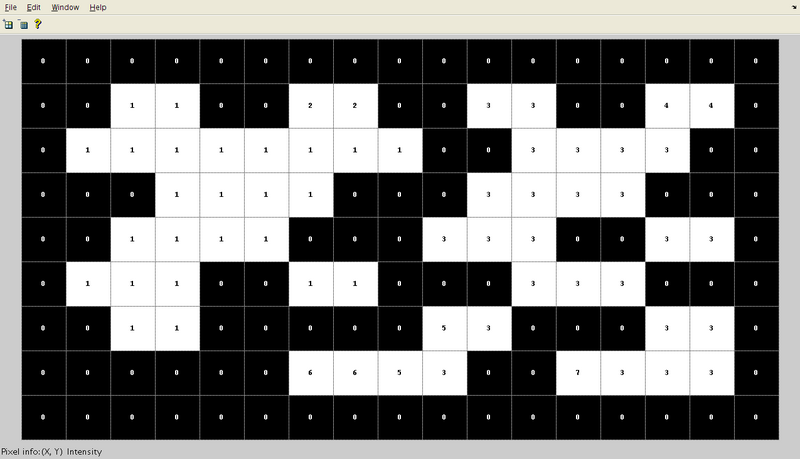
\includegraphics[scale=0.20]{Screenshot-Pixel_Region_(Figure_2).png}}
%     \end{figure}
% \end{frame}

% \begin{frame}{Algoritmo Two-pass / Double-pass}
%     \begin{figure}
%         \centering
%         \subfigure[Actualización de etiquetas]{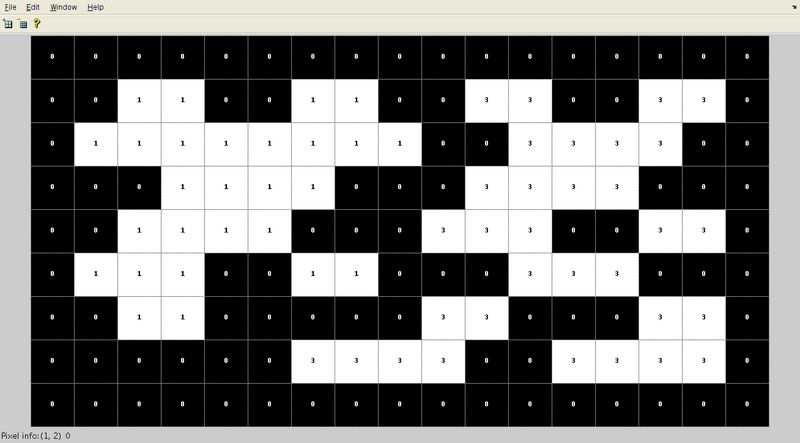
\includegraphics[scale=0.20]{Screenshot-Pixel_Region_(Figure_3).png}}
%         \subfigure[Identificación de regiones]{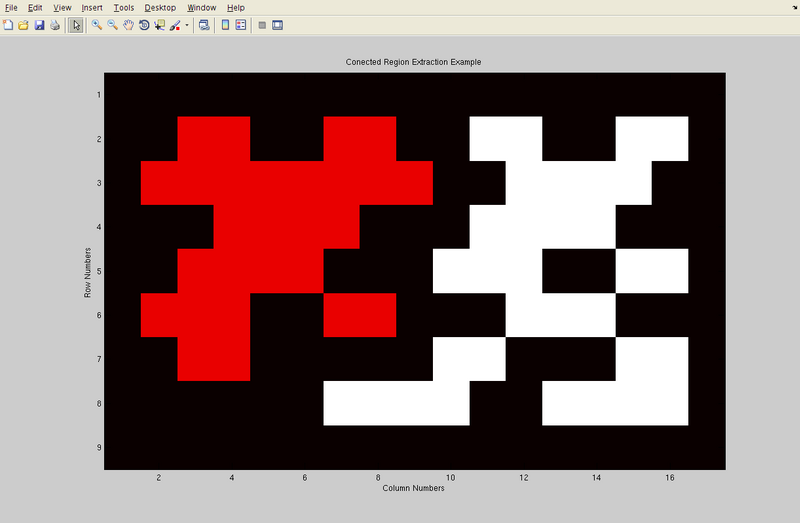
\includegraphics[scale=0.20]{Screenshot-Figure_1.png}}
%     \end{figure}
% \end{frame}

\begin{frame}{Referencias}
    \nocite{openacc_for_programmers}
    \nocite{parallel_openacc}
    \nocite{cuda}
    \printbibliography[heading=none]
\end{frame}

% \begin{frame}{Connected-Component Labeling}
%     %\begin{table}[ht]
%     \centering
%     %\subfloat[Decay Channels]{
%     %\rule{4cm}{3cm}
%     % \newcommand{\minitab}[2][l]{\begin{tabular}{#1}#2\end{tabular}}
%     %\renewcommand{\multirowsetup}{\centering}
%     \resizebox{13cm}{!}{\begin{tabular}{|c|c|} \hline
%             \multicolumn{2}{|c|}{Capa PHY para PCI Express}                                            \\
%             \hline
%             XIO1100 producido por Texas Instrument   & PX1011B producido por NXP                       \\
%             \hline
%                                                      &                                                 \\
%             Referencia de reloj de 100 MHz ó 125MHz. & Una sola línea de 2.5 Gbits/s.                  \\
%                                                      &                                                 \\
%             Bajo consumo de potencia.                & Posee un reloj de frecuencia máxima de 250 MHz. \\
%                                                      &                                                 \\
%             PCI Express 1.1 Compliant.               & Bajo consumo de energía.                        \\
%                                                      &                                                 \\
%             Un costo de \$9.7 la unidad.             & Costo por unidad de \$7.96.                     \\
%             \hline
%         \end{tabular}}
% \end{frame}

% \begin{frame}{Bloque general}
%     \begin{figure}
%         \centering
%         \includegraphics[scale=0.45]{bloque_general.pdf}
%     \end{figure}
% \end{frame}

\end{document}